\documentclass[a4paper]{article}

%use the english line for english reports
%usepackage[english]{babel}
\usepackage[USenglish]{babel}
\usepackage[utf8]{inputenc}
\usepackage{indentfirst}
\usepackage{graphicx}
\usepackage{verbatim}
\usepackage{listings}
\usepackage{minted}
\usepackage{float}
\usepackage{subcaption}
\usepackage{blindtext}
\usepackage{enumitem}
\usepackage{itemize}


\lstdefinestyle{myPrologstyle}
{
    language=Prolog,
    basicstyle = \ttfamily\color{blue},
    moredelim = [s][\color{black}]{(}{)},
    literate =
        {:-}{{\textcolor{black}{:-}}}2
        {,}{{\textcolor{black}{,}}}1
        {.}{{\textcolor{black}{.}}}1
}


\begin{document}

\setlength{\textwidth}{16cm}
\setlength{\textheight}{22cm}

\title{\Huge\textbf{Oolong}\linebreak\linebreak\linebreak
\Large\textbf{Relatório Final}\linebreak\linebreak
\linebreak\linebreak

\includegraphics[scale=0.1]{feup-logo.png}\linebreak\linebreak
\linebreak\linebreak
\Large{Mestrado Integrado em Engenharia Informática e Computação} \linebreak\linebreak
\Large{Programação em Lógica}\linebreak
}

\author{\textbf{Grupo 02:}\\ Gonçalo Moreno - up201503871 \\ Joao Almeida - up201505866 \\\linebreak\linebreak \\
 \\ Faculdade de Engenharia da Universidade do Porto \\ Rua Roberto Frias, s\/n, 4200-465 Porto, Portugal \linebreak\linebreak\linebreak
\linebreak\linebreak\vspace{1cm}}
\date{November 2017}
\maketitle
\thispagestyle{empty}

%************************************************************************************************

\newpage

    \section{Abstract}
    \normalsize

Our project consists in the 2 player board game called Oolong in Prolog.
 Throughout this report we will list and discuss the most important and
 critical design decisions, often aided with code snippets, for correctly
 implementing the game logic.
\newpage



%************************************************************************************************
\tableofcontents

%************************************************************************************************
%************************************************************************************************

%*************************************************************************************************
%************************************************************************************************

\newpage

%%%%%%%%%%%%%%%%%%%%%%%%%%
\section{Introduction}

This project was a assignment for the Curricular Unit PLOG at FEUP. \par
We were assigned with the implementation of the strategy game Oolong in Prolog.
It is interfaced over a terminal window and it was programmed in the recommended software,
 \textit{Sictus-Prolog}.
 \par
We designed this project to be as real and faithful representation of the real life counter-part and
also to have a clean and pleasant interface.

%%%%%%%%%%%%%%%%%%%%%%%%%%


\section{Oolong}
Oolong​ ​is​ ​an​ ​area-majority​ ​strategy​ ​game​ ​set​ ​in​ ​a​ ​Japanese​ ​tea​ ​house​ ​where​ ​the​ ​traditional
Oolong​ ​Tea​​ ​is​ ​being​ ​served.​ ​Each​ ​player​ ​represents​ ​a​ ​tea​ ​manufacturer​ ​trying​ ​to​ ​serve​ ​the​ ​most
of​ ​its​ ​brand,​ ​thus​ ​maximizing​ ​profit.​ ​Once​ ​a​ ​player​ ​has​ ​served​ ​5​ ​people​ ​at​ ​a​ ​table​ ​they​ ​have​ ​won
the​ ​favor​ ​of​ ​that​ ​table.​ ​Then,​ ​after​ ​a​ ​player​ ​has​ ​satisfied​ ​5​ ​tables​ ​they​ ​have​ ​won​ ​the​ ​favor​ ​of​ ​the
house​ ​and​ ​therefore​ ​the​ ​game.

\subsection{Setting​ ​the​ ​Game}
The board is comprised of 9 tables, each has 9 seats where the game tokens are played.
The arrangement of the tables should be similar to the layout of the seats of the tables. This way
each seat is like a map for the overall playing area, with each table corresponding to a seat
location. For easier setup and game play the different tables should be arranged in such a way that resembles a compass.

\subsection{Playing​ ​the​ ​Game}
The player with the black tokens goes first, and since the waiter begins on the center table
the player must serve tea on the center table. Depending on the seat the player decided to serve
the waiter shall be moved accordingly. Below is depicted the actions that occur in a single turn.
\begin{enumerate}
\item Serve tea by placing a token.
\item Move the waiter accordingly.
\item Possibly trigger a Special Action.
\end{enumerate}

\subsection{Serving​ ​Tea}
Every tea serving is directed as follows: The space on which tea is served indicates the
table where the next player shall serve their next tea. For example, if John serves the first tea of
the game on the N seat of the center table, Sarah must serve her tea on an empty space of the N
table.

\subsection{The​ ​Waiter}
To more easily track where the next player must play, the Waiter pawn is moved
immediately after a tea is served. Use the following guidelines to correctly place the Waiter.

\begin{enumerate}
\item Place the waiter on the tile which you have directed the next player to serve.
\item Place the waiter on the seat corresponding to the table you just played. For example, if
you served tea on the center table, place the Waiter on the center seat, covering an
already served tea if needed. Tea may not be served on the seat the waiter is on!
\end{enumerate}

\subsection{Special​ ​Actions}
A Special Marker was randomly assigned to each perimeter table during setup of the
game. These markers describe a special action that may be taken immediately once the needed
number of matching tea has been served on that table. Once a marker has been used it cannot be
used again for the rest of the game. If an action would trigger another action on a different tile
that action also occurs, but multiple special actions are resolved in the order they are triggered.
Below is a list of the markers and their effects.


\begin{figure}[H]
\centering
\minipage[t]{0.85\textwidth}
  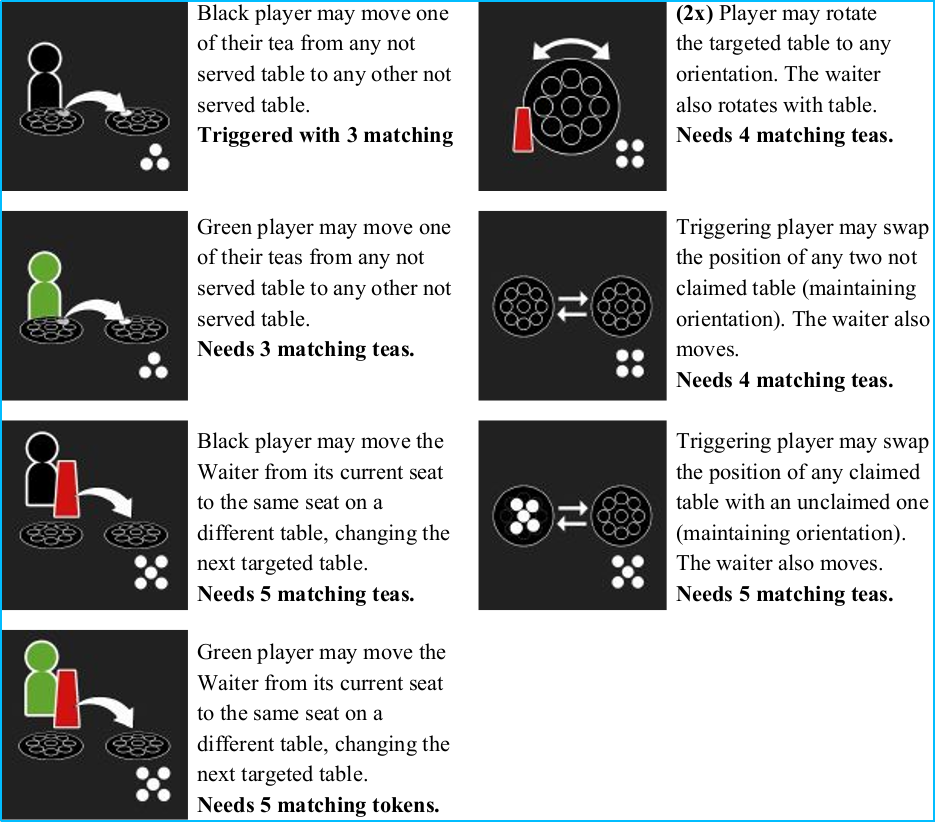
\includegraphics[width=\linewidth]{specials.png}
  \caption{Specials list.}\label{fig:specials}
\endminipage\hfill

\end{figure}

\subsection{Claiming a table}
Once a player has 5 served teas of their color on a table, they have claimed it. The table
remains in play, though once all empty seats have been served it is considered complete. If any
play (including special actions) should require a player to serve their tea on a completed table,
they instead choose any seat on any other incomplete table to serve their tea (it is generally a
poor strategic move to direct your opponent to a completed tile).


\subsection{Winning}
Once a player has claimed 5 tables they immediately win the game. It is not necessary to
fill every space on the tiles to complete the game.

%%%%%%%%%%%%%%%%%%%%%%%%%%


\newpage



\section{Game Logic}

\subsection{Game State Representation}
Oolong is a board game where positions are relevant, so we believe a list of lists is ideal
to represent the game state internally, where the index of the element in the list represents the
table and seat in which the token is to be placed. So, taking into account the picture below, the
element at the array in the position (3,3) represents the North seat at the North table.

\begin{figure}[H]
\centering
\minipage[t]{0.25\textwidth}
  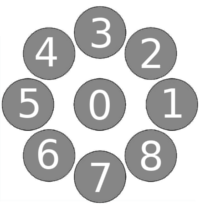
\includegraphics[width=\linewidth]{gameboard.png}
  \caption{Table Representation.}\label{fig:table_rep}
\endminipage\hfill
\end{figure}


\begin{listing}[H]
    \caption{Game Board Representation.}
    \label{Codigo:cod_board}
    \begin{minted}{prolog}

createSeats([], M, M).      %Stop if 2nd args = 3rd arg meaning max elems reached
%Creates the seats of a table
createSeats([H|T], N, M) :-
    N < M,                                  %add elements until max elements is reached
    N1 is N+1,                          %keep track of added element
    H = '.',                                %element to add
    createSeats(T,N1,M).    %recursive call

createTables([], M, M).

createTables([Head|Tail], 9, M) :-
    M1 is M-2,
    assignSpecials(Head, 0, M1),
    createTables(Tail, M, M).

%Creates the tables of the game
createTables([H|T], N, M) :-
    N \= 9,
    N < M,
    N1 is N+1,
    M1 is M-1,
    createSeats(H,0,M1),
    createTables(T, N1, M).

\end{minted}

\end{listing}
\newpage
The specials Actions are randomly attributed to each table. These are stored in a separate array from the tables,
this array is the last element of the regularly used Board variable. It is an array of 8 elements, each position
representing a table, starting from table 1 since table 0 has no special. Therefore the special present at index 0
is associated with the table 1, special at index 1 to table 2 and so forth.

\renewcommand\listingscaption{Code}

\begin{listing}[H]
    \caption{Specials assignment.}
    \label{Codigo:cod_special}
    \begin{minted}{prolog}
assignSpecials(Specials, Index, Size) :-
    assignSpecials(Specials, Index, Size, _).

assignSpecials([], Index, Index, _).
assignSpecials([Head|Tail], Index, End, SpecialsCopy) :-
    Index < End,
    Index1 is Index+1,
    repeat, %repeat until a new random is generated
        random(0, End, Special),
        (Index == 0 ; \+ member(Special, SpecialsCopy)),

    push(Special, SpecialsCopy, NewSpecials),
    Head = Special,
    assignSpecials(Tail, Index1, End, NewSpecials).

\end{minted}

\end{listing}

When the conditions for each special action are met the special action triggers immediately in accordance with the game rules.

\subsection{Board Visualization}

We have associated the character '.' with an empty space, 'X' and 'O' characters represent the two different players.
Furthermore the waiter when in an empty space is represented with a 'W', when it is on top of a 'X' token it is represented
with a '\%' and on top of a 'O' with a '@'.


\begin{figure}[H]
\centering

\minipage{0.4\textwidth}%
  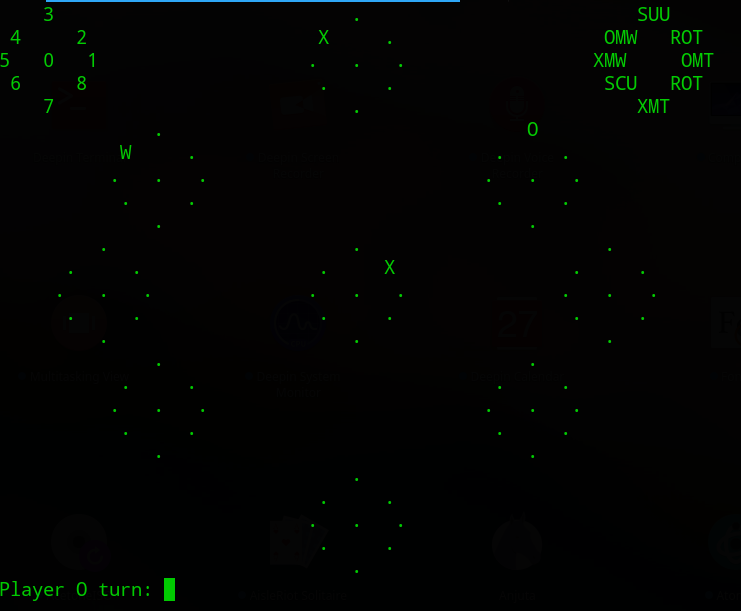
\includegraphics[width=\linewidth]{game.png}
  \caption{Game Interface.}\label{fig:game}
\endminipage \vspace{10mm} \hfill

\end{figure}

The Special Actions that are assigned to each table are displayed in the top right corner with a abbreviated name.
List of abbreviations and corresponding action: \vspace{1mm}

 \begin{itemize}
    \item X Player move tea (XMT).
    \item O Player move tea (OMT).
    \item X Player move Waiter (XMW).
    \item O Player move Waiter (OMW).
    \item Rotate table (ROT).
    \item Rotate table (ROT).
    \item Swap both not claimed (SUU).
    \item Swap claimed with unclaimed (SCU).
\end{itemize}

\subsection{Board Evaluation}

In order to correctly decide and implement plays and turns we used many board evaluation rules the most basic and simple are:

        \begin{listing}[H]
            \caption{At predicative for accessing tables and seats.}
            \label{Codigo:cod_at}
            \begin{minted}{prolog}
at(Elem,0,[Elem|_]).
at(Elem,Index,[_|Tail]) :-
    Index1 is Index - 1,
    Index > 0,
at(Elem,Index1,Tail).

    \end{minted}

    \end{listing}


        \begin{listing}[H]
        \caption{Find predicative mostly used for finding the waiter and empty seats.}
        \label{Codigo:cod_find}
        \begin{minted}{prolog}
find(_, _, Start1, []) :-
    Start1 = -1.
find(Elem, Start, Start1, [Elem|_]) :-
    Start1 = Start.
find(ElemToFind, Start, End, [_|Tail]) :-
    End \== -1,
    Index1 is Start+1,
    find(ElemToFind, Index1, End, Tail).

        \end{minted}

        \end{listing}


        \begin{listing}[H]
        \caption{Count predicative used for counting tokens on a table.}
        \label{Codigo:cod_count}
        \begin{minted}{prolog}

count([],_,0).
count([Head|Tail], Head, Total) :-
    count(Tail, Head, Total1),
    Total is 1+Total1.
count([Head|Tail], Elem, Total) :-
    Head \= Elem,
    count(Tail, Elem, Total).

        \end{minted}

        \end{listing}


These are used by many parts of the game, they are what we would call low level.
More complicated and higher level ones are used for triggering specials moves and determining tables
with a majority of token we have the following:

        \begin{listing}[H]
        \caption{Check Special, needed to trigger a special move.}
        \label{Codigo:cod_chekspecial}
        \begin{minted}{prolog}
checkSpecial(Board, Table, Seat, 0, TeaToken, NewBoard, NewSeatNumber, AI) :-
    TeaToken == 'X',
    moveOneToOther_3(Board, Table, TeaToken, NewBoard1, AI),
    handleWaiter(NewBoard1, Seat, NewBoard, NewSeatNumber).

checkSpecials(Board, Table, Seat, TeaToken, NewBoard, NewSeatNumber, AI) :-
    Table \= 0,
    at(Specials, 9, Board),
    Table1 is Table - 1,
    at(Special, Table1, Specials),
    checkSpecial(Board, Table, Seat, Special, TeaToken, NewBoard, NewSeatNumber, AI).
        \end{minted}

        \end{listing}

        \begin{listing}[H]
        \caption{Count Tables with a majority}
        \label{Codigo:cod_major}
        \begin{minted}{prolog}

countMajorTables(_, _, 9, PreviousTotal, NewTotal) :-
    NewTotal = PreviousTotal.
countMajorTables(Board, TeaToken, Index, PreviousTotal, NewTotal) :-
    Index1 is Index+1,
    at(BoardTable, Index, Board),
    countTableTokens(BoardTable, TeaToken, 0, 0, Total),
    (Total > 4 -> NextTotal is PreviousTotal+1 ; NextTotal is PreviousTotal+0),
    countMajorTables(Board, TeaToken, Index1, NextTotal, NewTotal).

        \end{minted}

        \end{listing}


With all of these we were able to implement most of the game's logic. From determining a valid move,
to check if a special move can be activated or if the game has ended.


\subsection{Turns}

The game loop will each turn evaluate the predicate \textit{turn(+TeaToken, +Table, +Board, -NewBoard, -NewTable)}
 which will ask the player for a seat validate it and change the Board accordingly, will also check and trigger any special moves.
  After this the board will be displayed
  and the other player will have its turn.

    \begin{listing}[H]
            \caption{Turn predicative.}
            \label{Codigo:cod_turn}
            \begin{minted}{prolog}
turn(TeaToken, CurrTableNumber, Board, NewBoard, NewTableNumber) :-
    play(CurrTableNumber, NewTableNumber1, SeatNumber, TeaToken, Board),
    serveTea(Board, NewTableNumber1, SeatNumber, TeaToken, NewBoard1),
    checkSpecials(NewBoard1, NewTableNumber1, SeatNumber, TeaToken, NewBoard, NewTableNumber, 0),
    drawBoard(NewBoard).

    \end{minted}

    \end{listing}


\subsection{End Game Verification}
 Each game loop iteration the predicative \textit{endCondition} will be evaluated. It will check for 5 tables being owned by the same Player. If this condition is met it will
  display a message saying who won the game.

\renewcommand\listingscaption{Code}

\begin{listing}[H]
    \caption{End Game Verification.}
    \label{Codigo:cod_end}
    \begin{minted}{prolog}
endCondition(Board, TeaToken) :- %  For player X
    countMajorTables(Board, TeaToken, 0, 0, Total),
    Total > 4,
    write('Congratulations Player'), write(TeaToken), write(' you have won.'), nl,
    halt.

\end{minted}

\end{listing}

\subsection{AI}
    When the AI is playing the game loop will call the predicative \textit{aiTurn} which will in turn get a valid seat
    from the predicative \textit{aiPlay} and play it, if the table is full it will call \textit{aiEndPlay} that will also get a random table
    .Both the table and seats are randomly choosen.

\begin{listing}[H]
    \caption{Predicatives for generating a AI move.}
    \label{Codigo:cod_ai}
    \begin{minted}{prolog}

aiPlay(CurrTableNumber, NewTableNumber, SeatNumber, Board) :-
    at(BoardTable, CurrTableNumber, Board),
    find('.', 0, FreeIndex, BoardTable),
    (
    FreeIndex \= -1 ->
        aiNormalPlay(CurrTableNumber, SeatNumber, Board), assignValue(CurrTableNumber, NewTableNumber)
        % gets random seat
        ;
        aiEndPlay(NewTableNumber, SeatNumber, Board)
        % gets random seat and table
    ).

aiTurn(TeaToken, CurrTableNumber, Board, NewBoard, NewTableNumber) :-
    write('AI '), write(TeaToken), write(' turn:'),
    aiPlay(CurrTableNumber, NewTableNumber1, SeatNumber, Board),
    serveTea(Board, NewTableNumber1, SeatNumber, TeaToken, NewBoard1),
    checkSpecials(NewBoard1, NewTableNumber1, SeatNumber,  TeaToken, NewBoard, NewTableNumber, 1),
    drawBoard(NewBoard).

\end{minted}

\end{listing}


%%%%%%%%%%%%%%%%%%%%%%%%%%
\section{User Interface}

The code responsible for interfacing with the user is located in the module/file 'io.pl'.
It's a combination of 3 menus and the game interface.

\begin{figure}[H]
\centering
\minipage[t]{0.23\textwidth}
  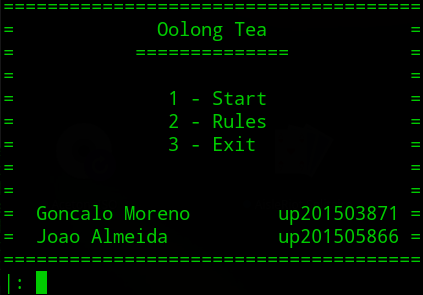
\includegraphics[width=\linewidth]{menu_inicial.png} \hspace{0.5cm}
  \caption{Inicial Menu.}\label{fig:menu_inicial}
\endminipage \hspace{2mm}
\minipage[t]{0.23\textwidth}
  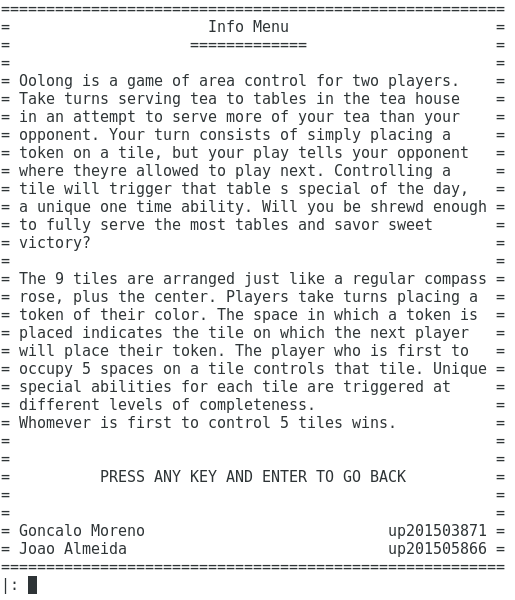
\includegraphics[width=\linewidth]{menu_info.png} \hspace{0.5cm}
  \caption{Rules Menu.}\label{fig:menu_info}
\endminipage \hspace{2mm}
\minipage[t]{0.23\textwidth}%
  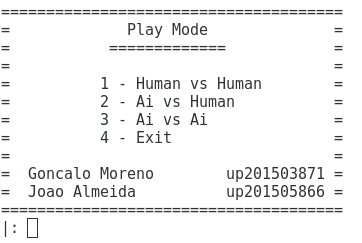
\includegraphics[width=\linewidth]{menu_play.png}\hspace{0.5cm}
  \caption{Game Options.}\label{fig:menu_play}
\endminipage\hfill


\end{figure}

\lstset{emph={%
   {:-}%
     },emphstyle={\color{red}\bfseries\underbar}%
}%

\newpage

%%%%%%%%%%%%%%%%%%%%%%%%%%
\section{Conclusion}
When we started this project we had very basic knowledge about logic programming and Prolog and at times
it was challenging to shift to a completely different style of programming and problem solving.
Nevertheless after overcoming plenty of difficulties and completing this game we came to the realization
that logic programming does have its advantages and use cases, especially when it comes to strategy games.
\par
When it comes to the state of the final game, there are some improvements that could be made the AI could be better,
in its current state it only plays the game randomly. Also there are some code smells that stem from the imperative programming
mindset.


\clearpage




\iffalse %%%NOT USED

\addcontentsline{toc}{section}{Bibliografia}
\renewcommand\refname{Bibliografia}
\bibliographystyle{plain}
\bibliography{myrefs}


\newpage
\appendix
\section{Game Code}

\fi  %%%NOT USED



\end{document}
